\documentclass[tikz]{standalone}
\usepackage{tikz}
\usetikzlibrary{fit}
\usepackage{tkz-graph}

\begin{document}
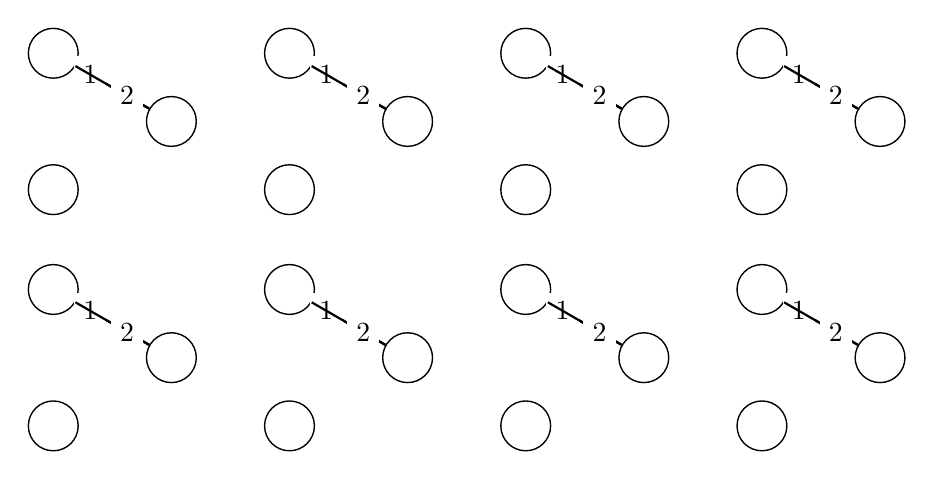
\begin{tikzpicture}[scale=1]
		%\tikzset{LabelStyle/.style= {draw,font = \small}}
		\GraphInit[vstyle=Normal]
		\SetVertexNoLabel
		\SetGraphUnit{1}
		\foreach \y in {0,3}{
			\foreach \x in {0,3,6,9}{
				\begin{scope}[xshift=\x cm,yshift=\y cm]
					\Vertices{circle}{a,b,c}
					%\Edge(a)(b)
					%\Edge(a)(c)
					%\Edge(b)(c)
					
					\Edge[label={1},style={pos=0.2,fill=red}](b)(a)
					\Edge[label={2},style={pos=0.7,fill=blue}](b)(a)
					%\Edge[label=1,style={pos=0.2}](a)(c)
					%\Edge[label=1,style={pos=0.2}](b)(c)
				\end{scope}
			}
		}
\end{tikzpicture}
\end{document}